\documentclass[a4paper,10pt]{article}
\usepackage[utf8x]{inputenc}

%opening
\title{Informe tarea algoritmos probabilísticos}
\author{María Andrea Cruz Blandón \and Edgar Andrés Moncada Taborda \and Luis Felipe Vargas Rojas}

\begin{document}

\maketitle

\section{N-Reinas - Las Vegas}

En un experimento de 8-Reinas realizado 1000 veces se obtuvo el siguiente resultado:
\begin{itemize}
 \item Promedio de probabilidad de éxito, el cual se obtuvo a partir de las probabilidades parciales de cada uno de los 1000 intentos es: $0.3077625$. A continuación se muestras las gráficas 
relacionadas con las probabilidades obtenidas, en una observamos como fueron las probabilidades en cada uno de los intentos y en el orden en que sucedieron, y en la otra veremos los intentos
ordenados por el valor de la probabilidad, en ésta podemos observar que el algoritmo tienen inclusos momentos en que en el primer intento obtiene éxito.

\begin{figure}
 \centering
 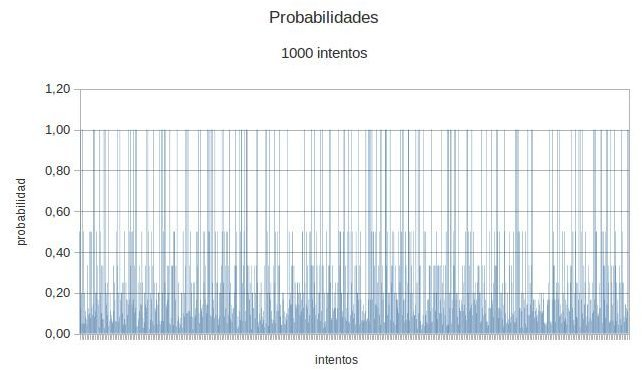
\includegraphics[scale=0.5]{promedios.jpg}
 \caption{Probabilidades de cada uno de los 1000 intentos}
 \label{fig:promedios}
\end{figure}

\begin{figure}
 \centering
 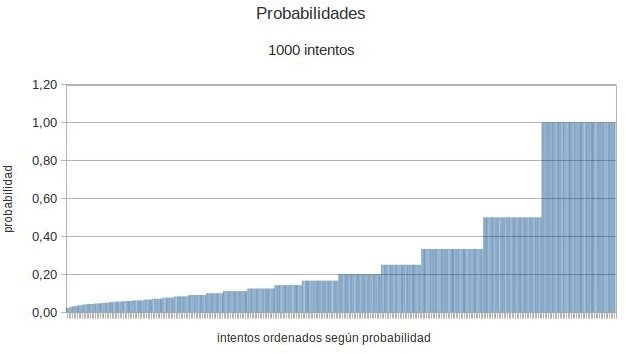
\includegraphics[scale=0.5]{probabilidadOrdenadas.jpg}
 \caption{1000 intentos ordenados por las probabilidades obtenidas}
 \label{fig:proOrden}
\end{figure}

\item Para analizar el tiempo esperado para el éxito, se contabilizó cuantas reinas se habían colocado en cada fracaso antes de que se diera dicho éxito. una vez tenemos este número procedemos a sacar
el promedio de los 1000 intentos para así obtener en número de reinas cuantas son necesarias para llegar al éxito. De este análisis se obtuvieron dos resultados, uno que en promedio son necesarios $6,577$ 
fracasos antes de encontrar el éxito aunque se alcanzaron numero de fracaso de hasta $39$. El segundo resultado tiene que ver con la cantidad de reinas que en promedio se insertaron en los fracasos
antes de dar con el éxito, aquí encontramos que en promedio (promedio de los promedios de los 1000 intentos) se necesitan $5,166$ reinas para encontrar el éxito.En la gráfica relacionada a la cantidad de reinas
promedio que se insertaron antes del éxito se observa cierta uniformidad. También debemos resaltar que 6 reinas insertadas conforma el $75\%$ de las reinas que se necesitan insertar y si este número
lo multiplicamos por el promedio de fracasos obtenemos que en promedio se están insertando $33,977$ reinas antes de encontrar el éxito.

\begin{figure}[h]
 \centering
 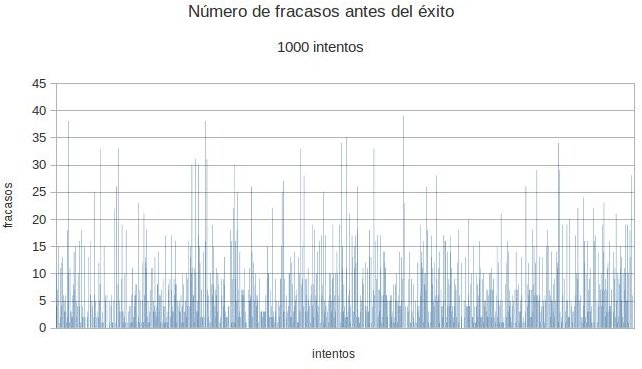
\includegraphics[scale=0.5]{fracasos.jpg}
 % fracasos.jpg: 642x369 pixel, 72dpi, 22.65x13.02 cm, bb=0 0 642 369
 \caption{Fracasos obtenidos antes del éxito en cada uno de los 1000 intentos}
 \label{fig:fracasos}
\end{figure}


\begin{figure}[h]
 \centering
 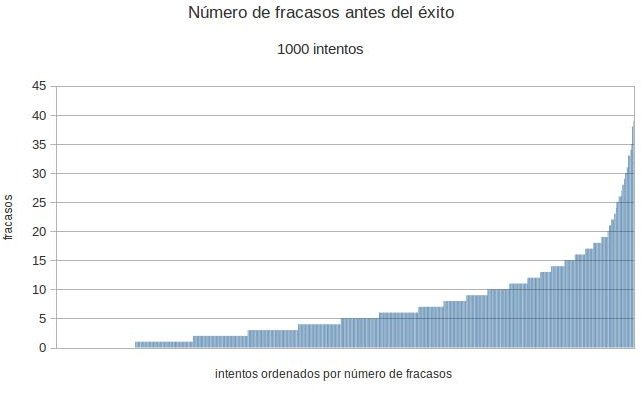
\includegraphics[scale=0.5]{fracasosOrden.jpg}
 % fracasosOrden.jpg: 642x393 pixel, 72dpi, 22.65x13.86 cm, bb=0 0 642 393
 \caption{Intentos ordeandos por numero de fracasos antes del éxito}
 \label{fig:fracasosOr}
\end{figure}


\begin{figure}[h]
 \centering
 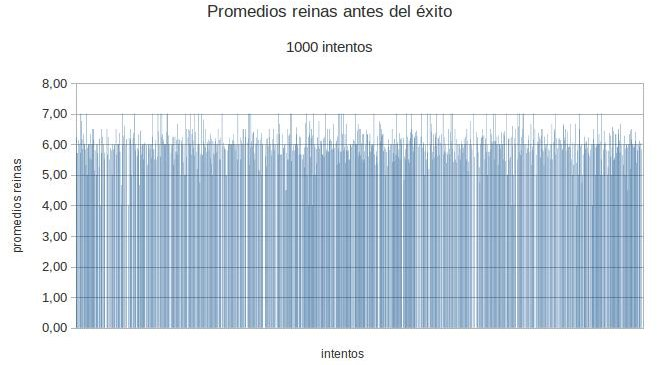
\includegraphics[scale=0.5]{reinaspromedio.jpg}
 % reinaspromedio.jpg: 657x365 pixel, 72dpi, 23.18x12.88 cm, bb=0 0 657 365
 \caption{Reinas promedio insertadas en cada fracaso antes de encontrar el éxito.}
 \label{fig:reinasprom}
\end{figure}

\item Para analizar el tiempo en que se demoraba en asignar posibles posiciones para luego elegir una aleatoriamente, se realizó el promedio por intento (fracaso-éxito), Así como se analizó
el número de reinas que se insertaron antes del éxito. Con lo anterior obtuvimos un promedio de $3,136$ posibles de los promedios de los 1000 intentos. En la gráfica podemos observar como este
promedio se mantiene con cierta uniformidad alrededor de 3 posibles.

\begin{figure}[h]
 \centering
 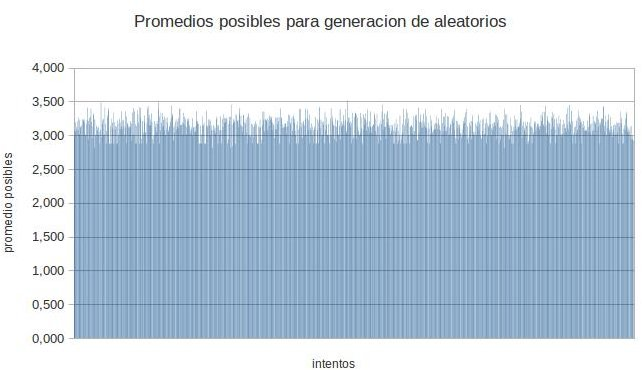
\includegraphics[scale=0.5]{promediosposibles.jpg}
 % promediosposibles.jpg: 816x1056 pixel, 72dpi, 28.79x37.25 cm, bb=0 0 816 1056
 \caption{Posibles antes de calcluar la posición aleatoria}
 \label{fig:posibles}
\end{figure}

\end{itemize}






\end{document}
